\section{Design of UP-SSO}
\label{sec:design}
\begin{figure}[t!]
  \centering
  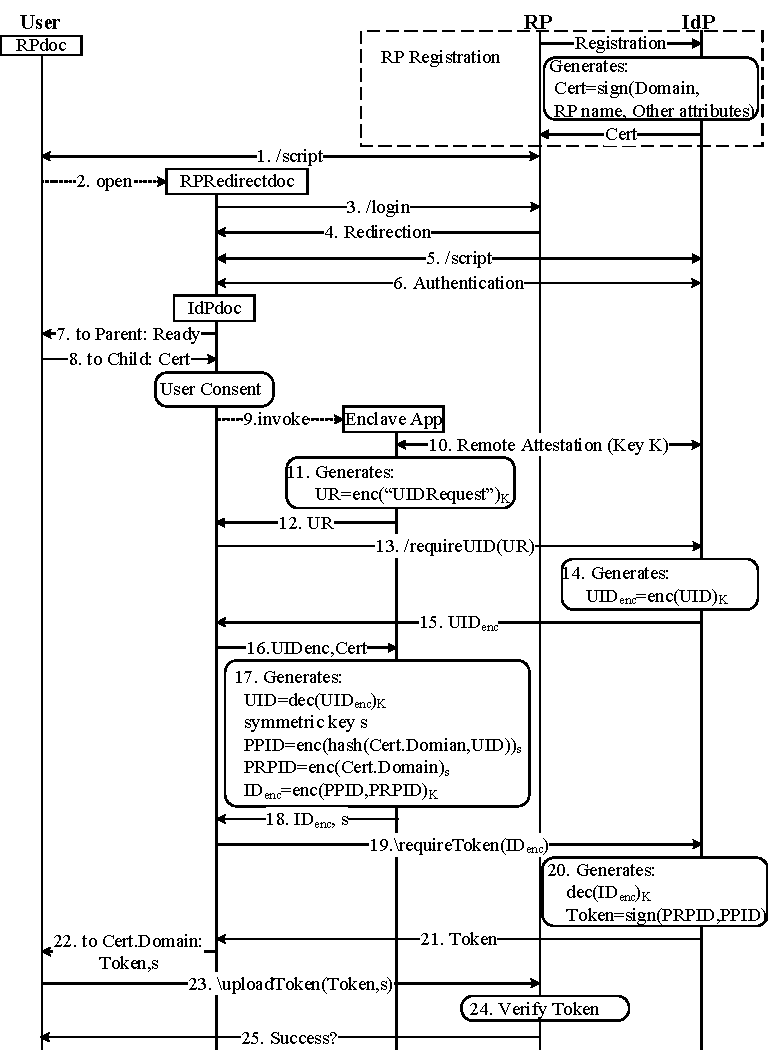
\includegraphics[width=\linewidth]{fig/sgx-sso.pdf}
  \caption{The protocol flow of UP-SSO.}
  \label{fig:UP-SSO}
\end{figure}
The UP-SSO is compatible with OIDC, besides that the IdP service is separated into user part and server part. 
The user agent (i.e., user-side IdP service) would obtain the UID from server part service, transform UID into the PPID, and encrypt the RPID and PPID with a one-time symmetric key to avoid IdP server digging out the RP's identity. As the enclave application is protected by SGX, it must not conduct any malicious behaviour. 
The server-side IdP service takes the responsibility of authenticating the user, retrieving the UID for each user, and issuing the identity token (i.e., the identity proof) consisted the privacy-preserving RP and user identifier.


\subsection{UP-SSO procedures}
\vspace{3mm}\noindent\textbf{RP Registration.} At the very beginning, RP needs to register its domain, RP name and other essential attributes at IdP, and obtains a signed Cert.  Thus, the  IdP can only provide the service to the qualified RP by checking the ownership of a Cert inside the enclave application.

Following, we provide the detailed protocol of UP-SSO.
The procedures of UP-SSO are depicted in detail in Figure~\ref{fig:UP-SSO}. It can be split into three phases, scripts downloading, PPID generation and identity token issuing. Here, we describe the details. 

\vspace{3mm}\noindent\textbf{Scripts downloading.} The scripts downloading phase is for the user’s browser to download the scripts from the RP and IdP servers. The scripts work as part of the user agent role.
\begin{itemize}
\item[1]The SSO process is started with the user's visit to an RP at her browser, and the browser downloads the RP script. The script is used to conduct the behaviour defined by RP on user side.
\item[2]The RP script opens a new window. 
\item[3]The newly opened window visits RP login endpoint.
\item[4]The user is redirected to the IdP server from RP login endpoint.
\item[5]The user retrieves the IdP script, which is used to deal with the interaction with IdP server, RP script and enclave application.
\end{itemize}
It must be noticed that, the user cannot visit IdP at step 2,3 directly because of the $Referer$ attribute in HTTP header. While the script in origin A opens a new window with origin B, the HTTP request to B's server will carry the key-value $Referer: A$. Therefore, the RP's domain is exposed to IdP. With HTML5, a special attribute for links in HTML was introduced, that the $ref="noreferrer"$ can be used to make $Referer$ header be suppressed. However, when such a link is used to open a new window, the new window does not have a handle on the opening window (opener) anymore. The handle is necessary for UP-SSO to transmit messages between RP and IdP scripts. So the redirection is adopted to avoid the HTTP header $Referer$ and make the handle of the opening window available. 


\vspace{3mm}\noindent\textbf{PPID Generation.} In this phase, IdP script invokes the enclave application to generate the PPID. 
\begin{itemize}
\item[6]At first, the IdP authenticates the user.
\item[7]After the IdP script is downloaded, it sends the ready signal to its opener (i.e., the RP window).
\item[8]RP script sends the RP's Cert back to IdP script. 
\item[9] The IdP script shows RP name to user to make sure the login is targeting to the correct RP, and then invokes the enclave application.
\item[10]The enclave application conducts remote attestation at its initialized execution. After the remote attestation, enclave application and IdP server share a symmetric key $K$.
\item[11]The enclave application generates the UID request (i.e., $UR$) by encrypting request information with $K$.
\item[12]$UR$ is sent to IdP script.
\item[13]Then the user starts the UID request to IdP.
\item[14]IdP encrypts $UID$ with $K$.
\item[15]IdP script receives encrypted $UID$ from IdP.
\item[16]IdP script transmits encrypted $UID$ and RP's domain to enclave application.
\item[17]The enclave application derives the $UID$ with $K$, verifies the Cert, achieves RP's domain from Cert, generates the symmetric key $s$, encrypts the RP's domain with key $s$ as the transformed RP ID (i.e., $PRPID$), encrypts the hash of RP's domain and UID as the $PPID$, and encrypts $PRPID$ and $PPID$ with $K$.
\item[18]Enclave application sends the encrypted IDs and $s$ to IdP script. 
\end{itemize} 
The PPID must be the encrypted hash of RP's domain and UID, instead of the plain digest. It avoids the IdP to find out multiple logins targeting the same RP or not, as the hash of same RP's domain would be always the same. 

Moreover, there are some types of parameters required in OIDC protocol to be carried in the SSO request, such as $response\_type$ and $scope$. In this paper, we would not mention these attributes, and only focus on the necessary parameters. 

\vspace{3mm}\noindent\textbf{Identity token issuing.} In this phase, IdP issues an identity token containing the encrypted $PPID$ and $PRPID$. And the RP verifies the token.
\begin{itemize}
\item[19]User sends the encrypted $PRPID$ and $PPID$ to IdP for identity token.
\item[20]The IdP server derives the $PRPID$ and $PPID$, signs the $token$ consisted of $PRPID$ and $PPID$ as the identity proof.
\item[21]IdP sends identity token to enclave application.
\item[22]The IdP script then sends the $token$ and $s$ to the origin RP's $Domain$ through $postMessage$.
\item[23]The RP script uploads the $token$ and key $s$ to RP server.
\item[24]The RP server firstly verifies the signature with IdP's public key, then generates the $PRPID$ with its domain and key $s$, and compared it with the one carried by $token$. If the two $PRPID$s are equaled, RP decrypts the user's account from $PPID$, and finds out the related user information in its database.
\item[25]RP returns the login result back to user.
\end{itemize} 
The origin in step 22 is essential for secure identity token transmitting.
It guarantees that only the script running in the RP window can receive the $token$, that avoids the man-in-the-middle attack.

